% ==============================================================================
% CAPÍTULO 4: DINÁMICA MULTIPARTÍCULA Y ESPACIO DE FASES
% ==============================================================================
\chapter{Dinámica Multipartícula, Espacio de Fases y Amortiguamiento Adiabático}

\section{Evolución del Paquete de Partículas en el Espacio de Fases}
Para caracterizar la estabilidad longitudinal del haz, se realizó el seguimiento discreto de un paquete de $N = 3000$ protones a lo largo de las 55 celdas del LINAC Álvarez. Las partículas se inyectaron a $T_0 = 3.0\text{ MeV}$ con distribuciones gaussianas ($\sigma_T = 15.0\text{ keV}$, $\sigma_\phi = 15.0^\circ$) centradas en la fase síncrona $\phi_s = -30^\circ$.

\begin{figure}[H]
    \centering
    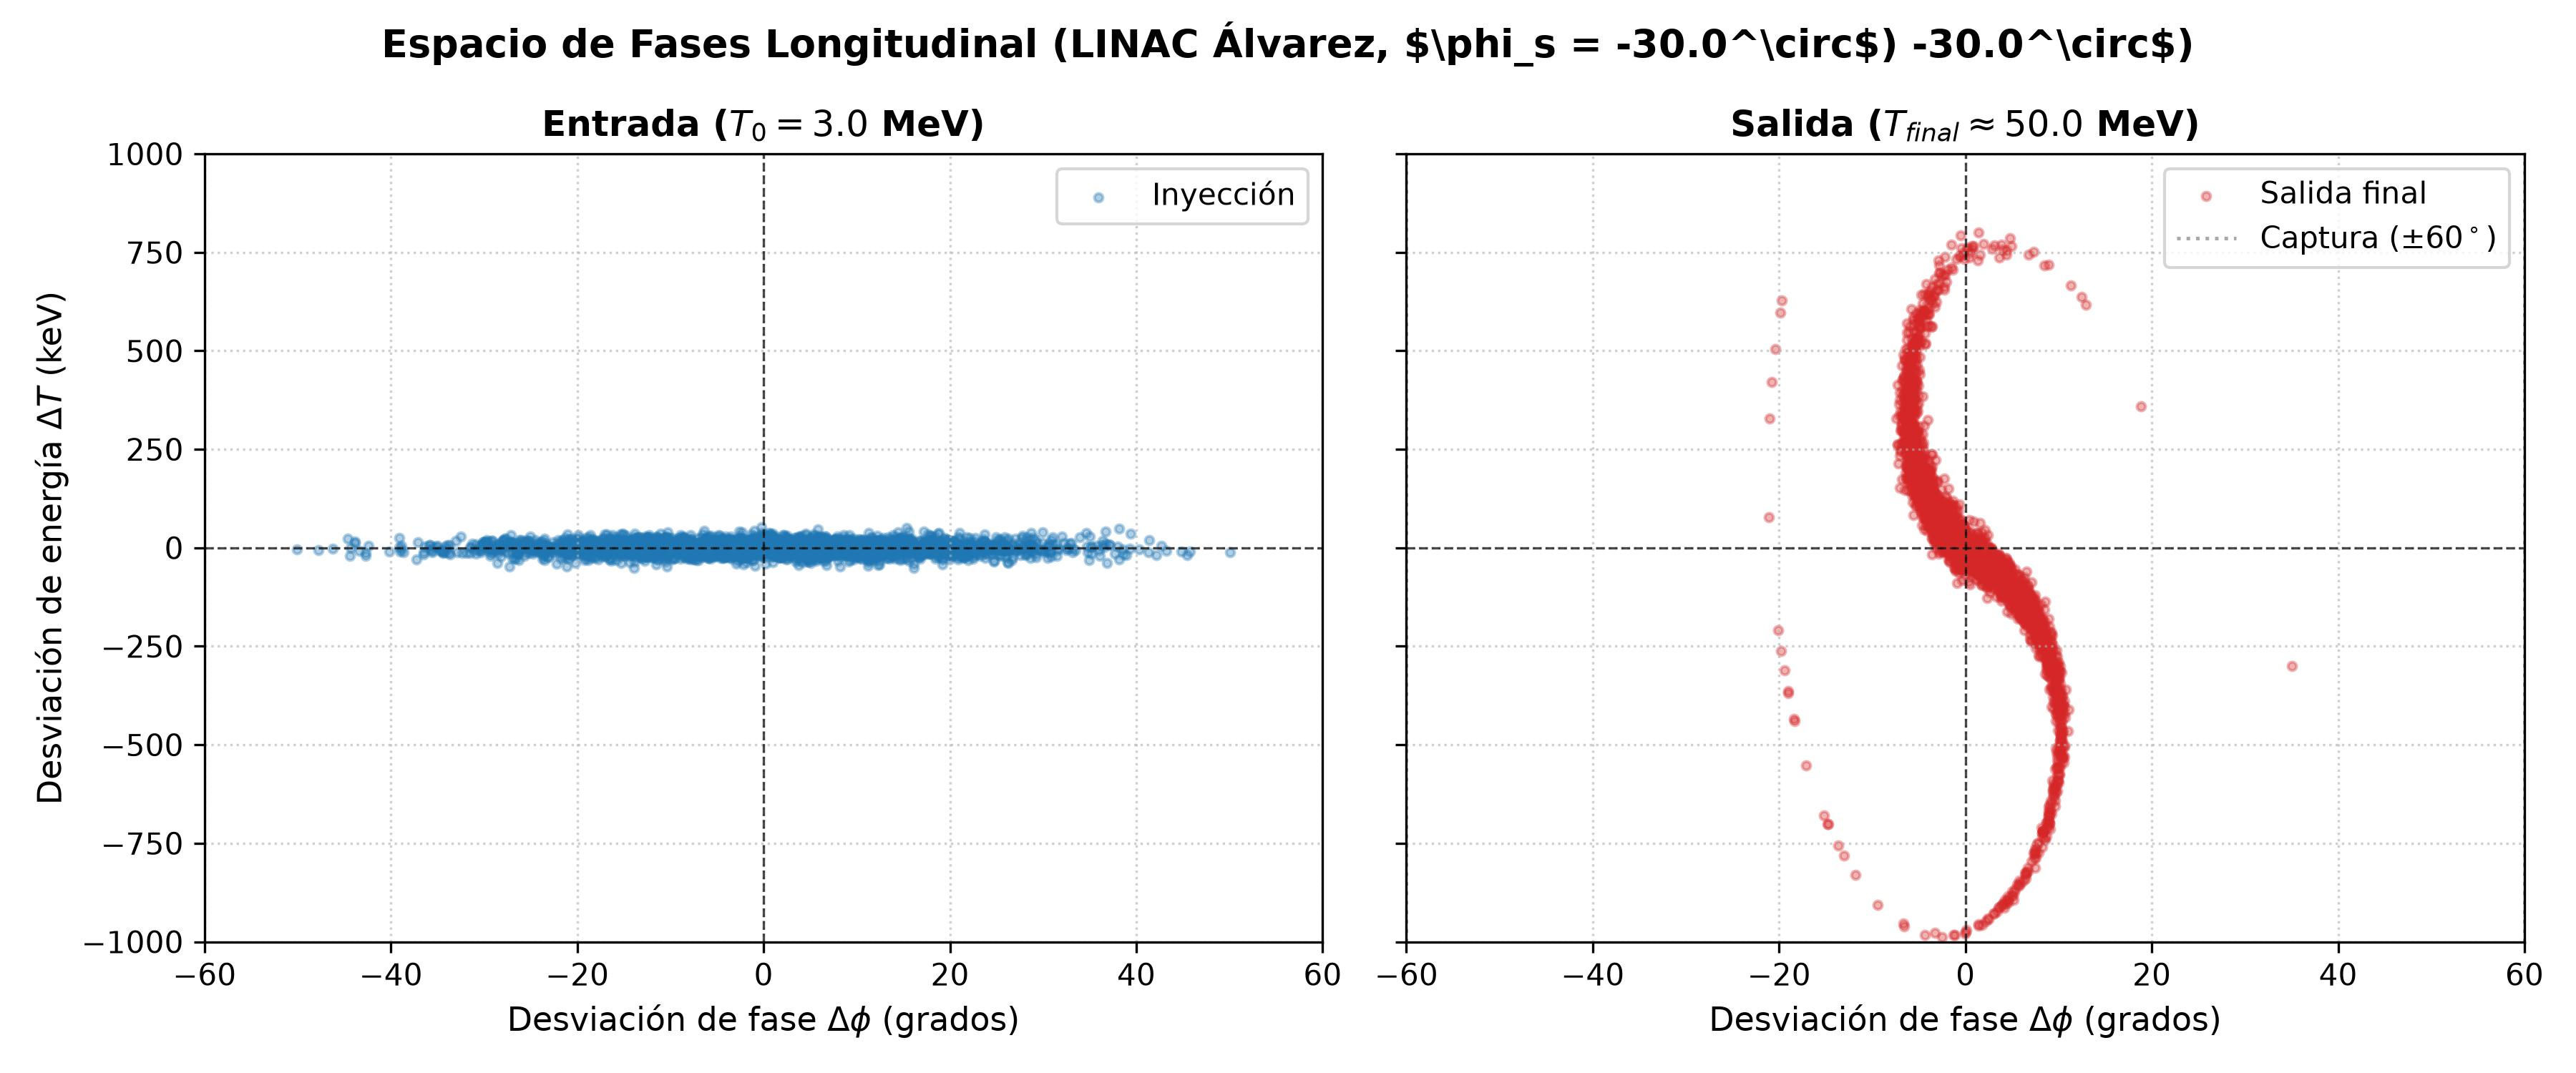
\includegraphics[width=0.88\textwidth]{figuras/fig02_espacio_fases.png}
    \caption{Rotación del haz de 3000 protones en el espacio de fases $(\Delta\phi, \Delta T)$ desde la inyección en Celda 1 (3.0 MeV) hasta la extracción en Celda 55 (50 MeV).}
    \label{fig:espacio_fases}
\end{figure}

Como se observa en la Figura \ref{fig:espacio_fases}, la distribución de partículas experimenta un movimiento de rotación coherente en el espacio de fases $(\Delta\phi, \Delta T)$ a medida que oscila alrededor del punto fijo síncrono. En la celda final (55), el $99.1\%$ de las partículas permanecen confinadas dentro de la región de estabilidad longitudinal.

\section{Demostración del Teorema de Liouville y Amortiguamiento Adiabático}
De acuerdo con el Teorema de Liouville, la emiteza longitudinal empaquetada debe mantenerse constante durante un proceso hamiltoniano sin pérdidas. Sin embargo, en coordenadas físicas $(\Delta\phi, \Delta T)$, el incremento sostenido del momento relativista del protón ($\beta\gamma$) produce el fenómeno de \textit{amortiguamiento adiabático}.

Las amplitudes de oscilación de la dispersión de fase ($\sigma_\phi$) y de la dispersión de energía ($\sigma_T$) evolucionan según las relaciones de proporcionalidad:
\begin{equation}
\sigma_\phi(n) \propto (\beta_n \gamma_n)^{-3/4}, \quad \sigma_T(n) \propto (\beta_n \gamma_n)^{3/4}
\end{equation}

\begin{figure}[H]
    \centering
    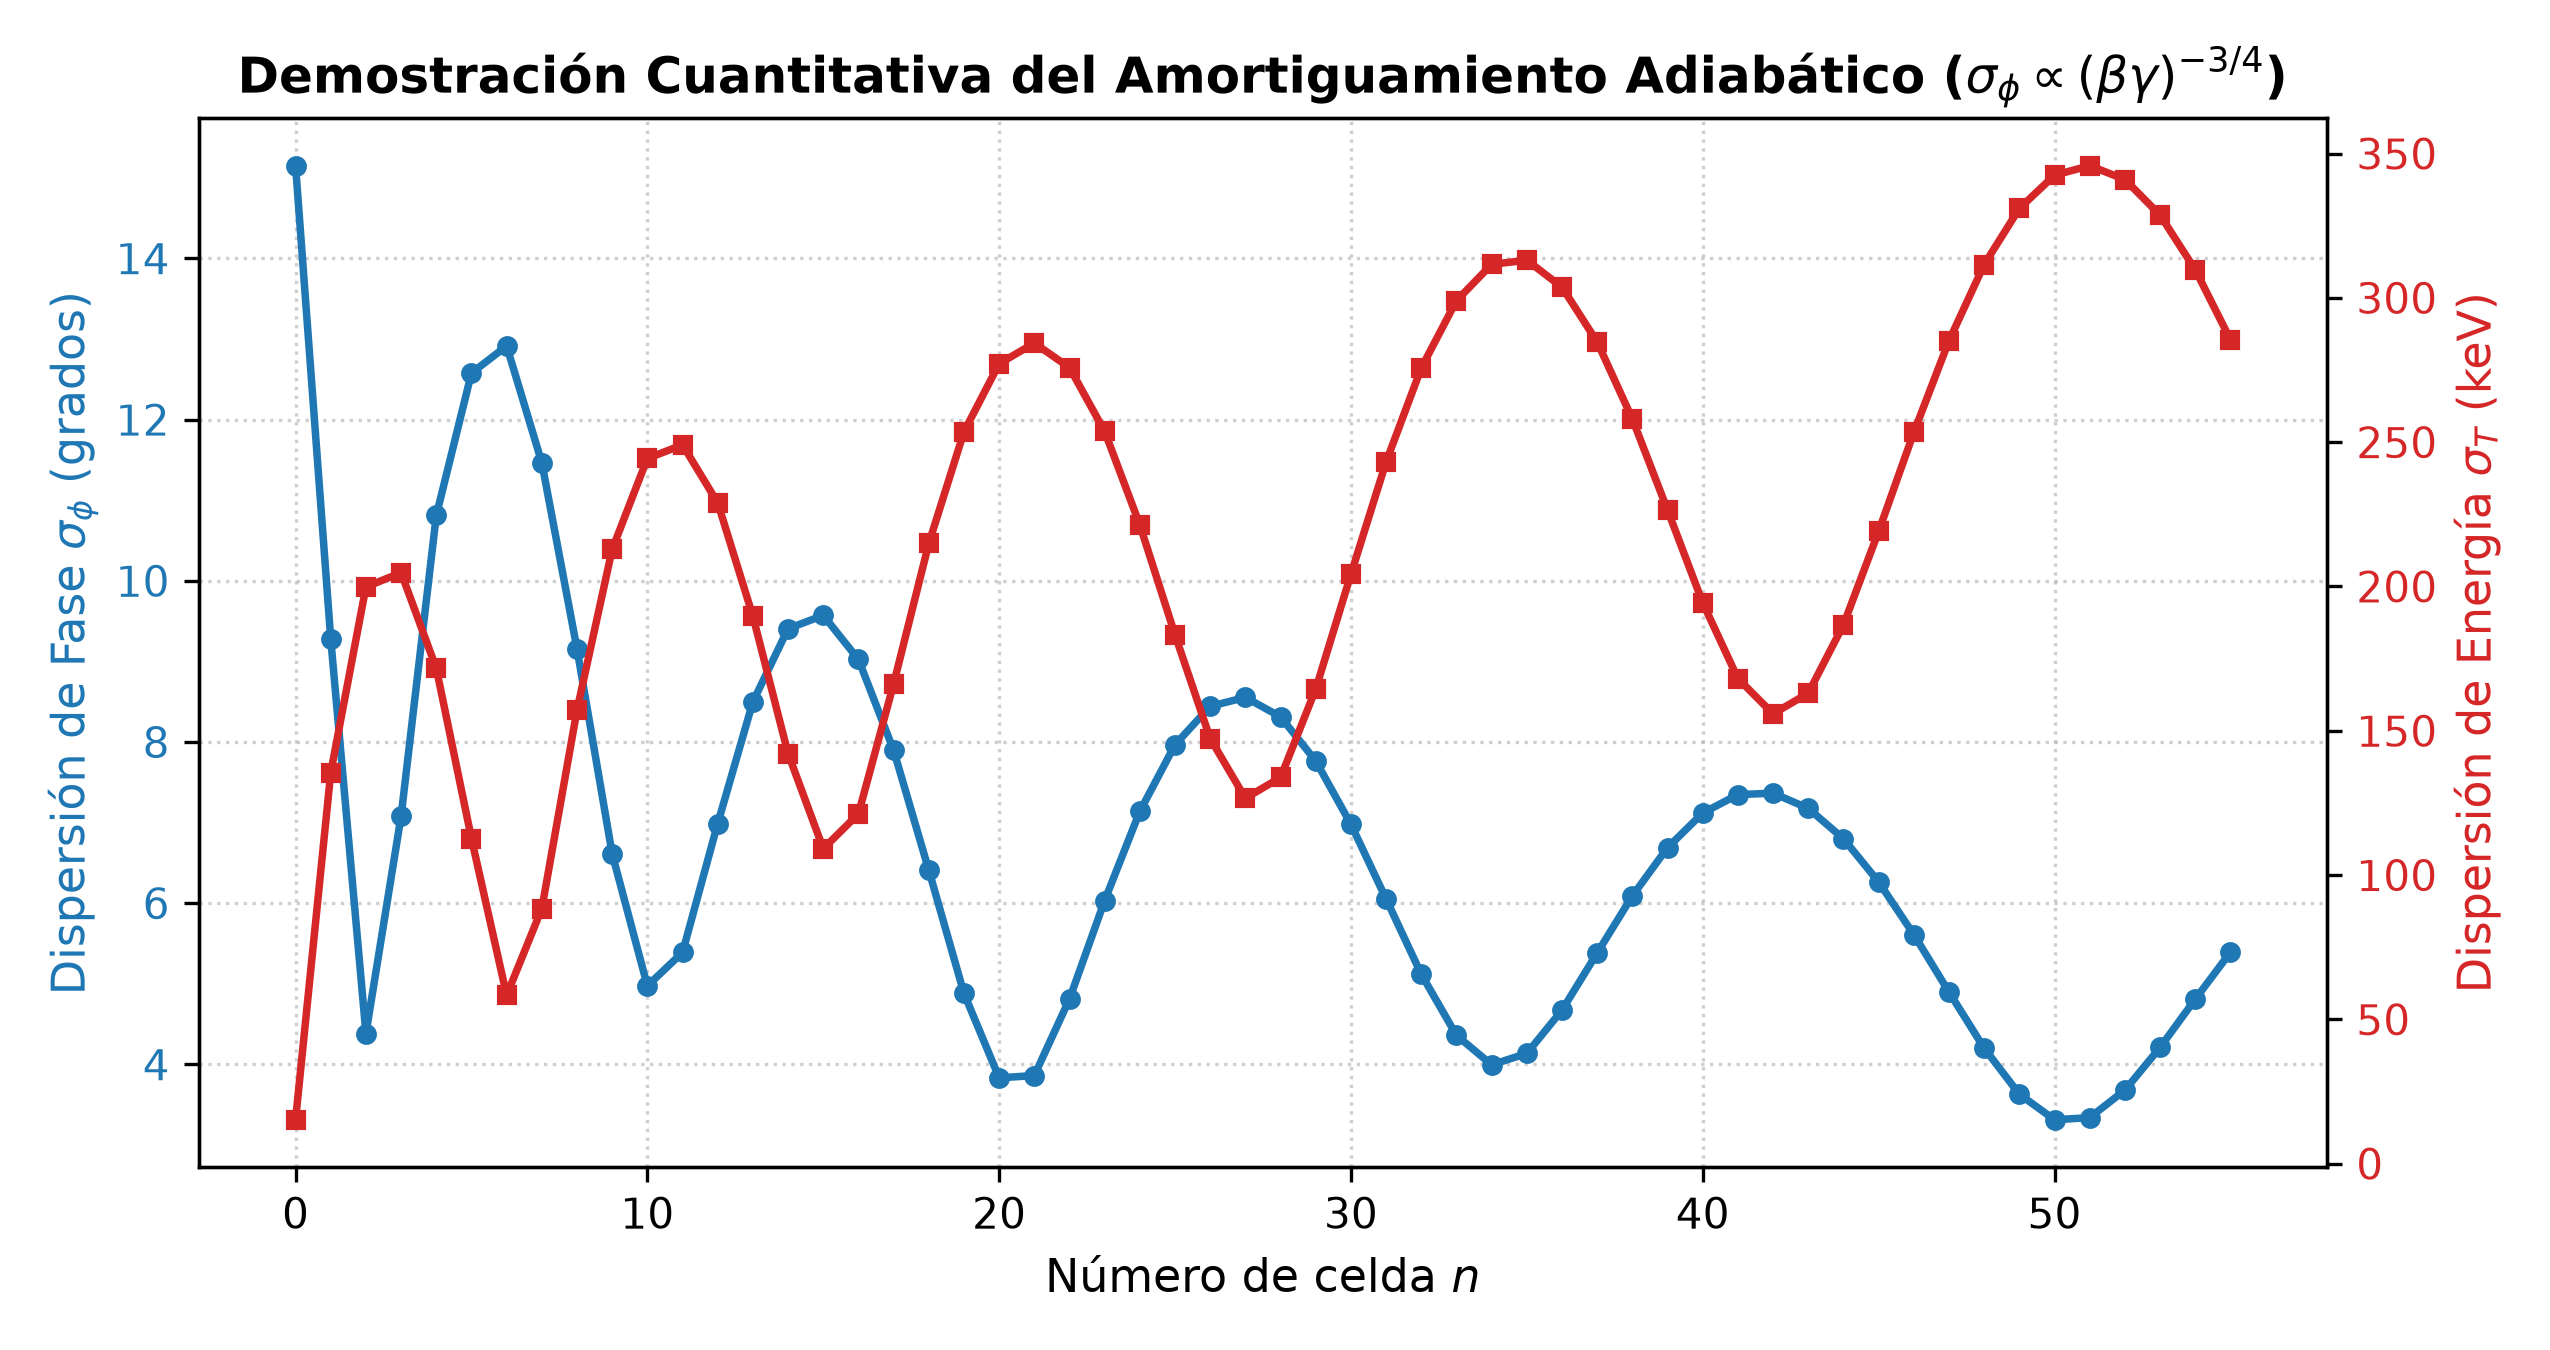
\includegraphics[width=0.88\textwidth]{figuras/fig07_amortiguamiento_cuantitativo.png}
    \caption{Evolución celda a celda del amortiguamiento adiabático: compresión de la dispersión de fase $\sigma_\phi$ (grados) frente a la expansión de la dispersión de energía $\sigma_T$ (keV).}
    \label{fig:amortiguamiento_cuantitativo}
\end{figure}

La Figura \ref{fig:amortiguamiento_cuantitativo} confirma cuantitativamente esta predicción teórica:
\begin{itemize}
    \item La dispersión estándar de fase $\sigma_\phi$ se comprime drásticamente desde $\sigma_{\phi, 0} = 15.19^\circ$ en la inyección hasta $\sigma_{\phi, 55} = 5.27^\circ$ en la extracción.
    \item La dispersión de energía $\sigma_T$ se expande desde $\sigma_{T, 0} = 15.15\text{ keV}$ hasta $\sigma_{T, 55} = 284.47\text{ keV}$, preservando el producto del área total en el espacio de fases.
\end{itemize}

\section{Mapa de Densidad 2D del Haz Extraído}
Para modelar las mediciones de los monitores de perfil longitudinal de intensidad de haz (*beam profile monitors*), en la Figura \ref{fig:densidad_emiteza} se presenta el mapa de densidad bidimensional (histograma 2D de frecuencia) del paquete en la Celda 55.

\begin{figure}[H]
    \centering
    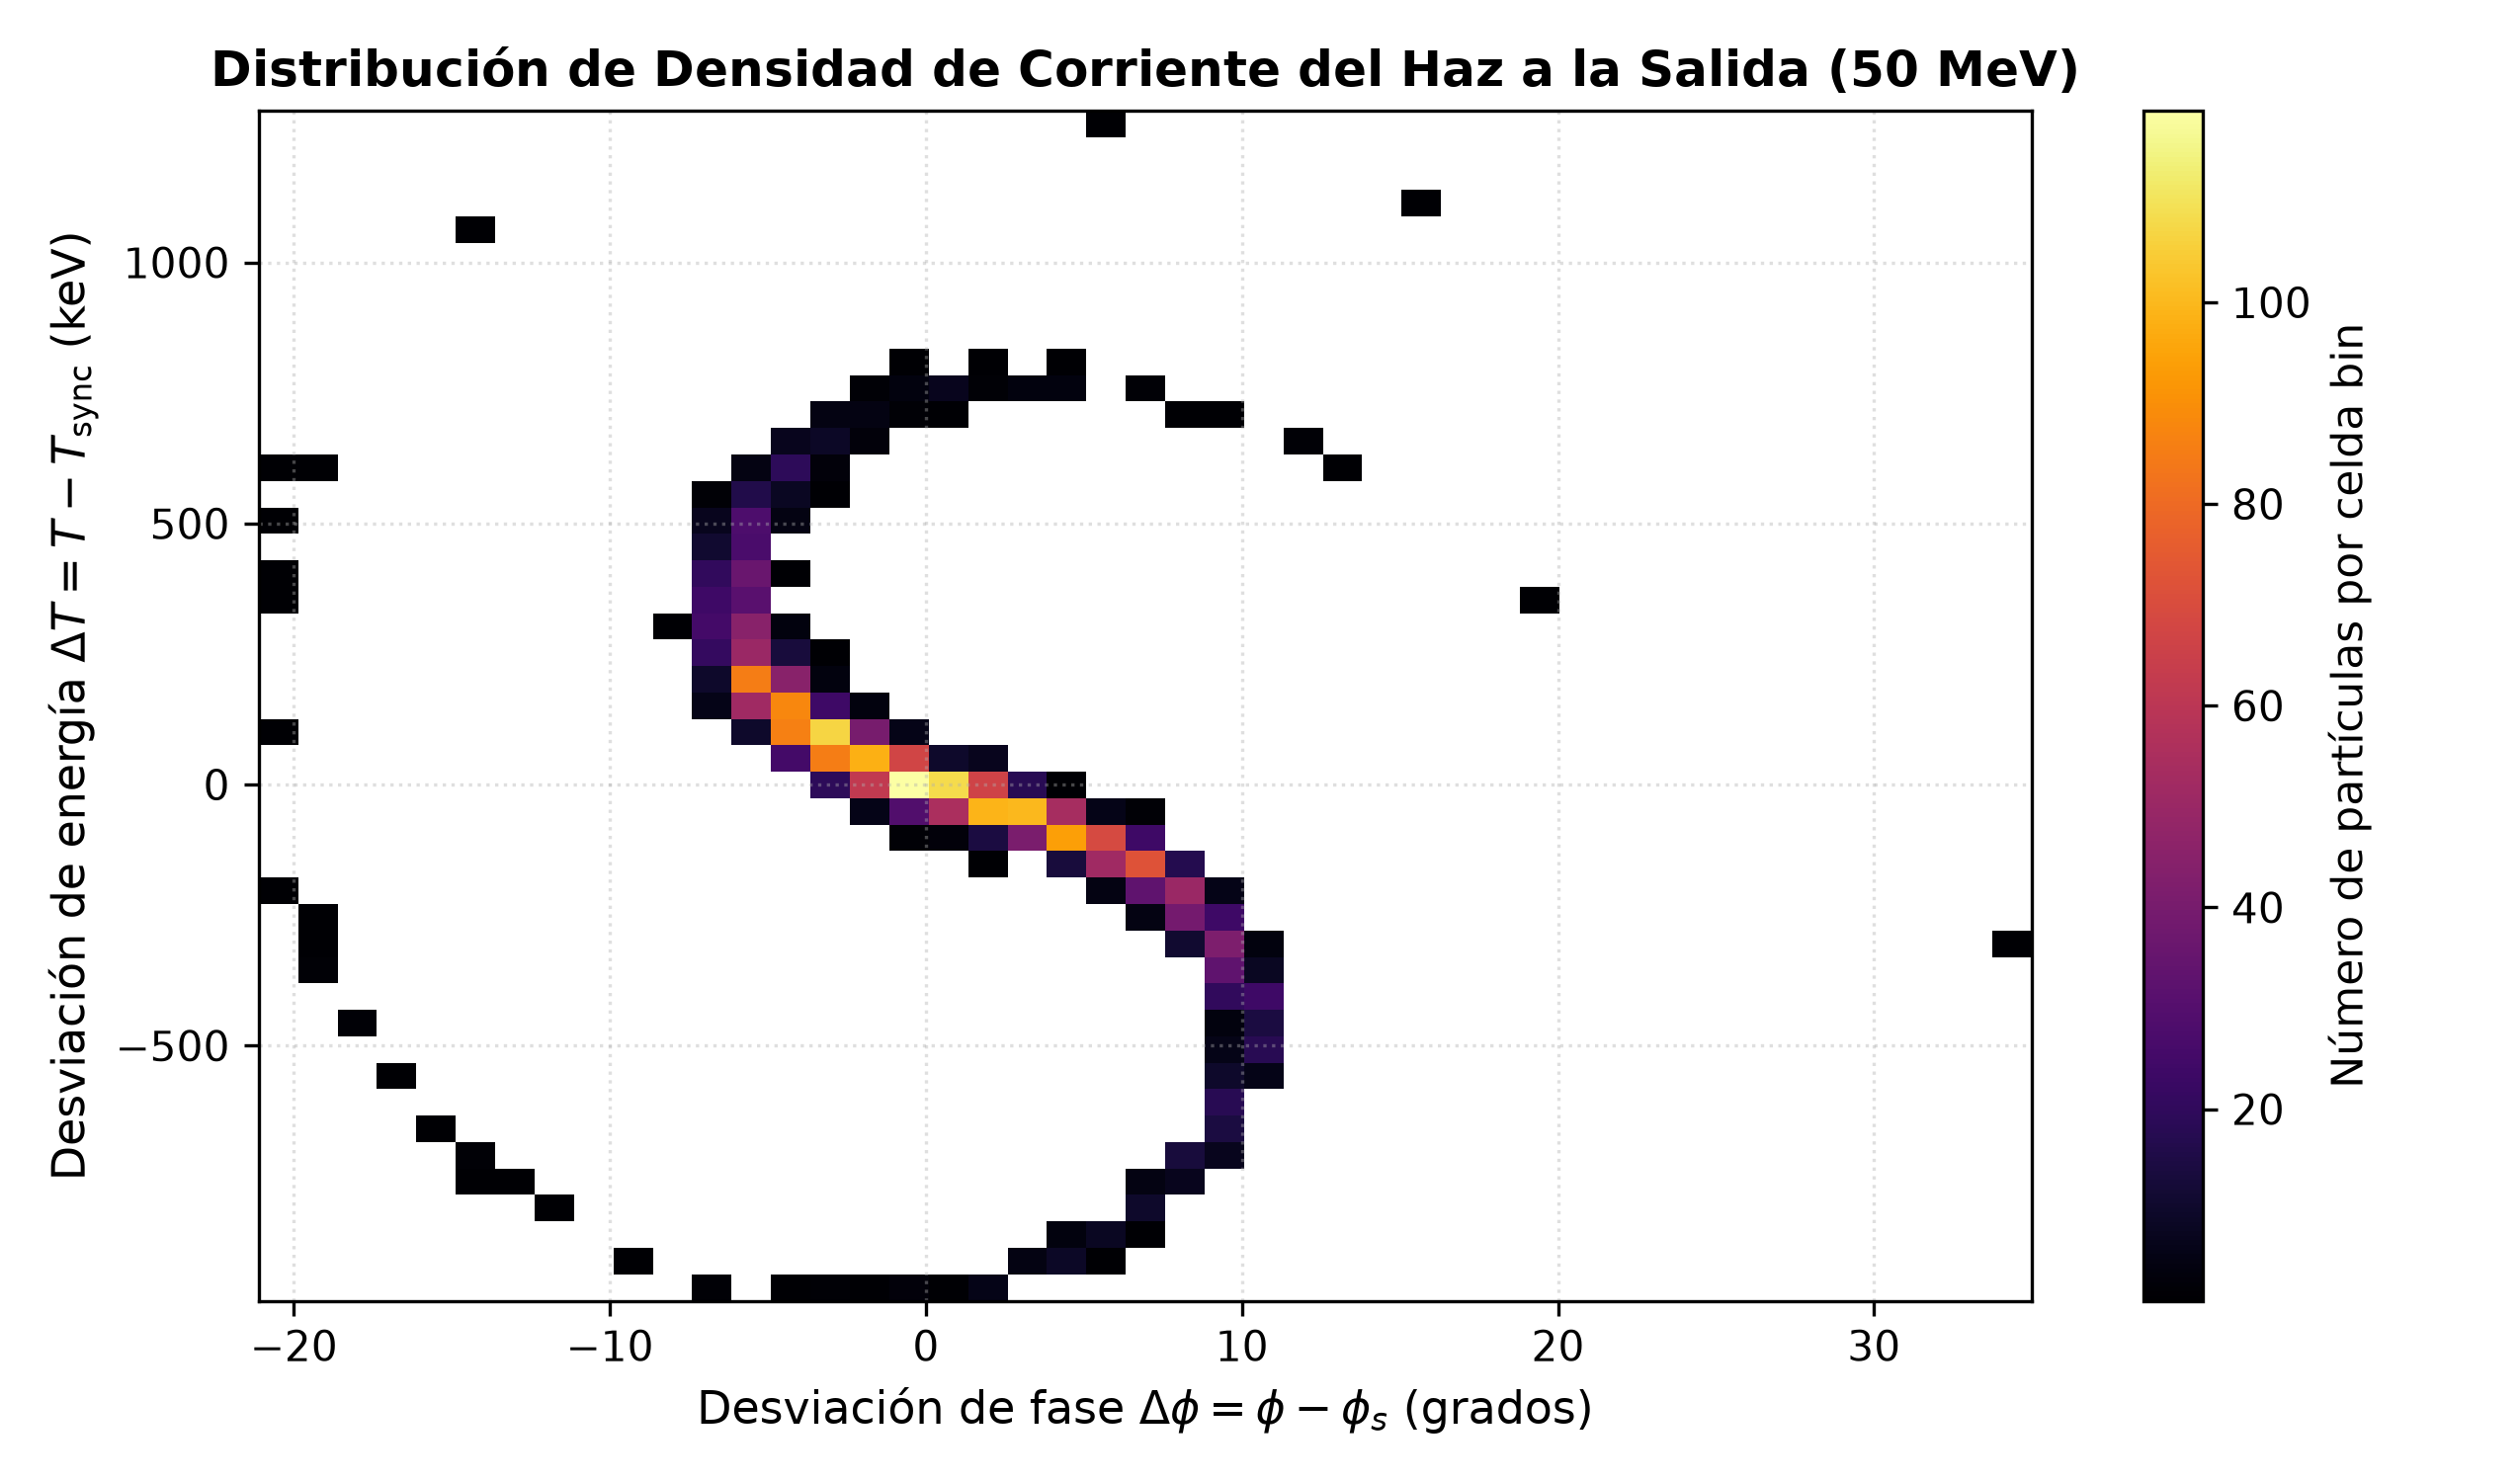
\includegraphics[width=0.85\textwidth]{figuras/fig10_densidad_emiteza_salida.png}
    \caption{Mapa de densidad 2D de emiteza del haz extraído (50 MeV) que permite distinguir el núcleo denso (*core*) del halo de partículas.}
    \label{fig:densidad_emiteza}
\end{figure}

El histograma bivariado en el plano $(\Delta\phi, \Delta T)$ permite distinguir con claridad el núcleo denso del haz (*core*, representado en regiones de alto conteo de partículas en color amarillo/blanco) rodeado por una distribución exterior de menor densidad correspondiente al halo longitudinal de difusión.